\setAuthor{Martne Rannut}
\setRound{lõppvoor}
\setYear{2023}
\setNumber{G 6}
\setDifficulty{6}
\setTopic{TODO}

\prob{Nõel vees}
Nõel massiga $m=\SI{0.5}{\g}$ ning pikkusega $l=\SI{6}{\cm}$ asetatakse aeglaselt vee pinnale. Millise nurga alla on veepind nõela juures horisontaalpinna suhtes paindunud? Vee pindpinevustegur $\sigma=\SI{72.8}{\mN\per\m}$ ja raskuskiirendus $g=\SI{9.81}{\m\per\s\squared}$. Üleslükkejõuga võib mitte arvestada.


\hint

\solu
\par
Ülesandes kirjeldatud olukord on ligikaudu näidatud joonisel. Veepind pisut kõverdub ning seeläbi pindpinevusjõuga tasakaalustab nõela raskusjõu. Pindpinevusjõud mõjub veepinna sihis kontaktpunktides (see ei pruugi olla tangentsiaalne nõela pinnaga nagu on joonisel näidatud, kuid ülesande lahendust see ei mõjuta). Kummalegi poolele nõelast mõjub jõud $\sigma \ell$. Kui pindpinevusjõu vektorid on horisontaali suhtes nurga $\alpha$ all, siis saame jõudude tasakaalust \(mg = 2 \sigma \ell \sin \alpha\). Kuna veepind on sama nurga all kui jõuvektorid, siis otsitav nurk on
\[
\alpha = \arcsin{\frac{mg}{2\sigma \ell}} \approx \SI{34}{\degree}.
\]
\begin{center}
  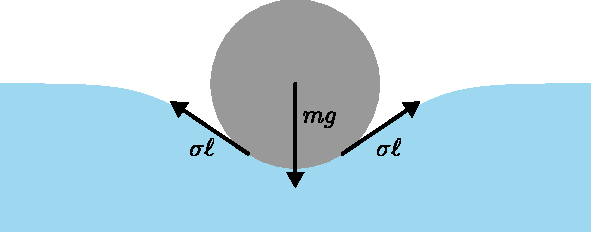
\includegraphics[width=9cm]{2023-v3g-06-sol.pdf}
\end{center}
\probend